\documentclass[a4paper,12pt]{article}
\usepackage[utf8]{inputenc}
\usepackage[spanish]{babel}
\usepackage{color}
\usepackage{parskip}
\usepackage{graphicx}
\usepackage{multirow}
\usepackage{listings}
\usepackage{vmargin}
\usepackage{datetime}
\newdate{date}{19}{10}{2017}
\graphicspath{ {imagenes/} }
\definecolor{mygreen}{rgb}{0,0.6,0}
\definecolor{lbcolor}{rgb}{0.9,0.9,0.9}
\usepackage{epstopdf}
\usepackage{float}


\setpapersize{A4}
\setmargins{2.5cm}       % margen izquierdo
{1.5cm}                        % margen superior
{16.5cm}                      % anchura del texto
{23.42cm}                    % altura del texto
{10pt}                           % altura de los encabezados
{1cm}                           % espacio entre el texto y los encabezados
{0pt}                             % altura del pie de página
{2cm}     

\lstset{
    tabsize=4,    
%   rulecolor=,
    language=[GNU]C++,
        basicstyle=\tiny,
        aboveskip={1.5\baselineskip},
        columns=fixed,
        showstringspaces=false,
        extendedchars=false,
        breaklines=true,
        prebreak = \raisebox{0ex}[0ex][0ex]{\ensuremath{\hookleftarrow}},
        frame=single,
        showtabs=false,
        showspaces=false,
        showstringspaces=false,
        identifierstyle=\ttfamily,
        keywordstyle=\color[rgb]{0,0,1},
        commentstyle=\color[rgb]{0.026,0.112,0.095},
        stringstyle=\color{red},
        numberstyle=\color[rgb]{0.205, 0.142, 0.73},
%        \lstdefinestyle{C++}{language=C++,style=numbers}’.
}


\begin{document}
\title{Práctica de Laboratorio 1}
\author{
Christofer Fabián Chávez Carazas \\
\small{Universidad Nacional de San Agustín de Arequipa} \\
\small{Escuela Profesional de Ciencia de la Computación} \\
\small{Computación Gráfica}
}
\date{\displaydate{date}}

\maketitle

\begin{enumerate}
 \item \textbf{Compile y ejecute el código de la pŕactica} 
 \begin{figure}[H]
  \centering
  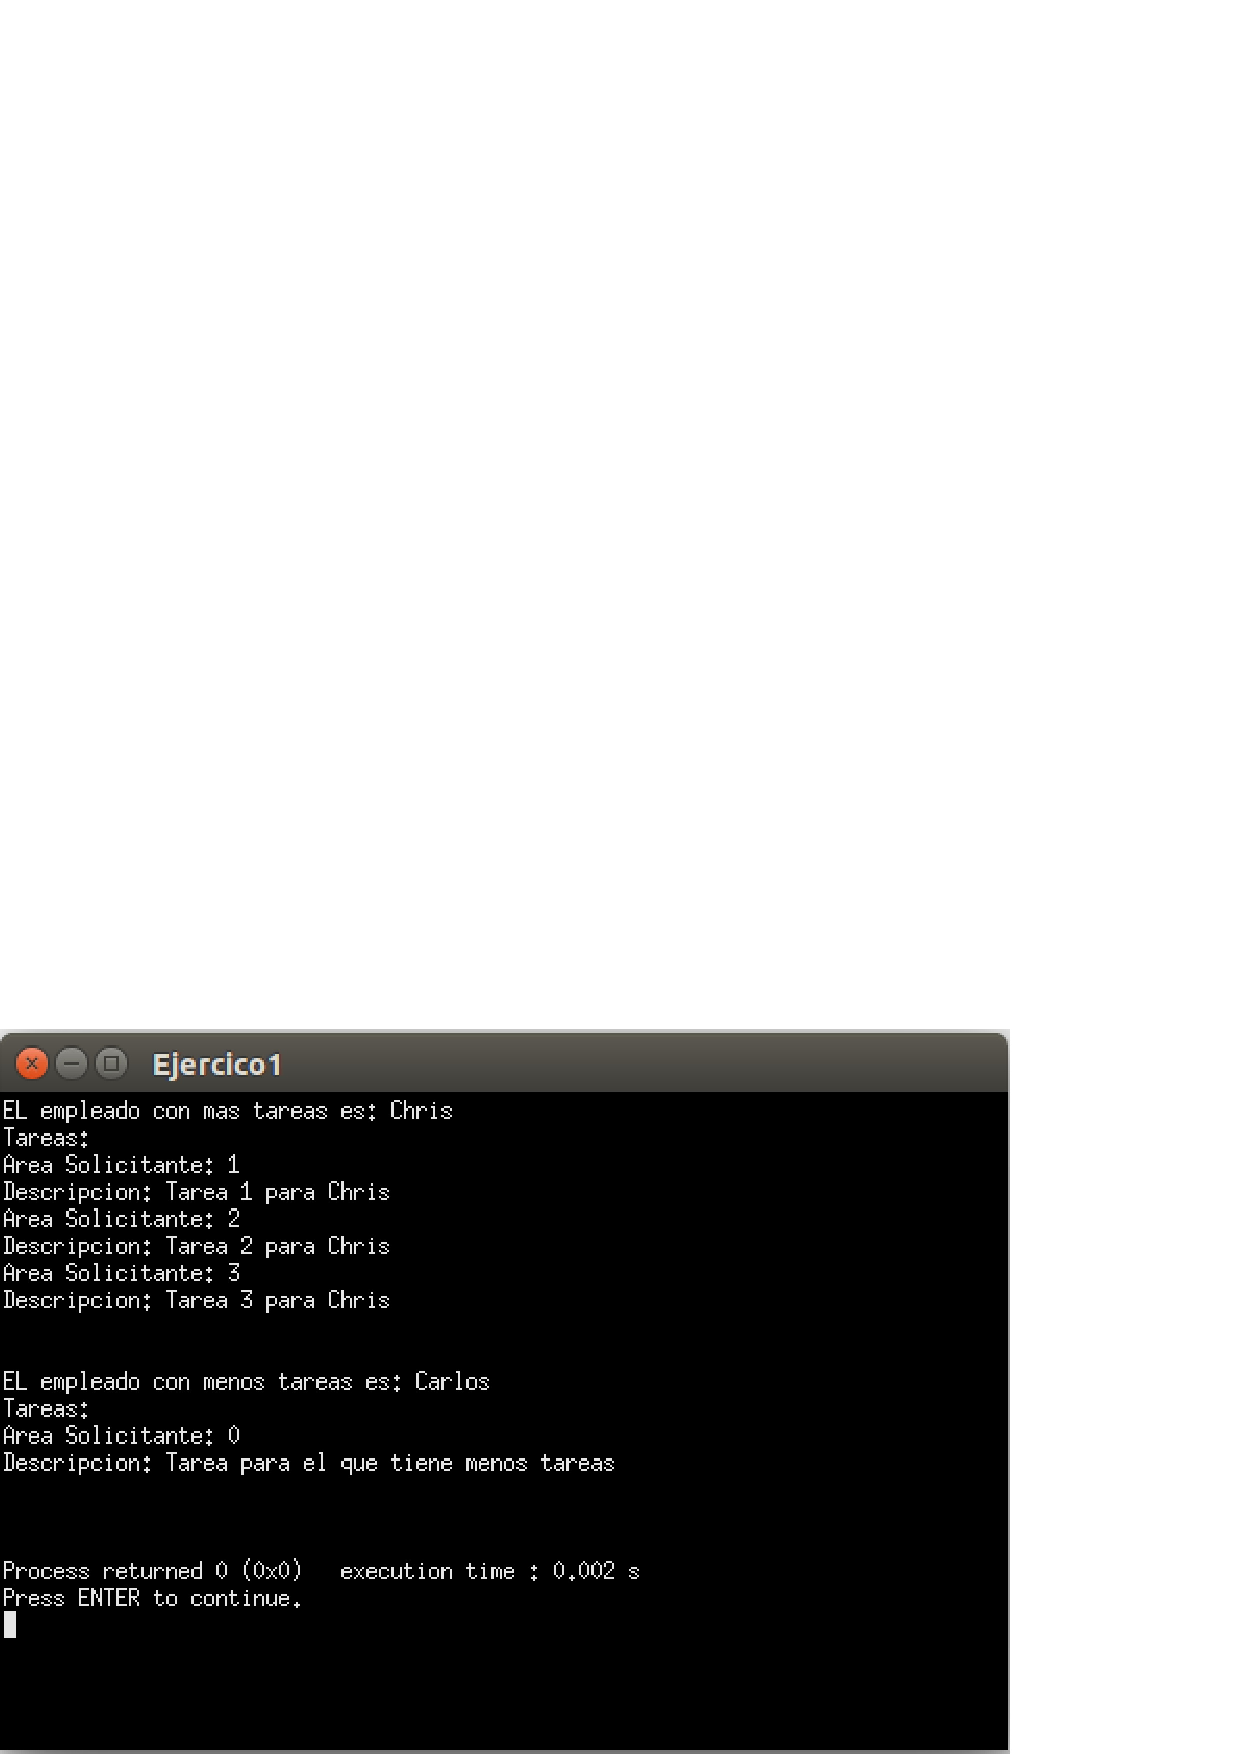
\includegraphics[scale = 0.5]{1.png}
  \caption{Resultado del programa}
 \end{figure}
 
 \item \textbf{Explique que función cumple cada línea de código}
 \begin{itemize}
  \item \textit{glClearColor:} Establece el color de la ventana de visualización.
  \item \textit{glMatrixMode:} Establece los parámetros de proyección.
  \item \textit{gluOrtho2D:} Define una matriz de proyección ortogonal 2D.
  \item \textit{glClear:} Borra la ventana de visualización.
  \item \textit{glColor3f:} Establece el color del segmento de línea.
  \item \textit{glBegin:} Inicio de un grupo de primitivas.
  \item \textit{glVertex2i:} Especifica la geometría del segmento de línea.
  \item \textit{glEnd:} Fin de un grupo de primitivas.
  \item \textit{glFlush:} Procesa las subrutinas de OpenGl.
  \item \textit{glutInit:} Inicializa GLUT.
  \item \textit{glutInitDisplayMode:} Establece el modo de visualización
  \item \textit{glutInitWindowPosition:} Establece la posición de la esquina superior izquierda de la ventana de visualización.
  \item \textit{glutInitWindowSize:} Establece el ancho y la altura de la ventana de visualización.
  \item \textit{glutCreateWindow:} Crea la ventana de visualización.
  \item \textit{glutDisplayFunc:} Envía los gráficos a la ventana de visualización.
  \item \textit{glutMainLoop:} Muestra todo y espera. 
 \end{itemize}

 \item \textbf{Modifique los parámetros de proyección ortogonal en función del tamaño de la ventana. Comente sus resultados.}
 
 Con los parámetros dados en la práctica, la línea aparece en casi toda la ventada de visualización, si se cambian esos parámetros en
 función del tamaño de la ventana, entonces la línea aparece en una porción de la ventana de visualización.
 
 \begin{figure}[H]
  \centering
  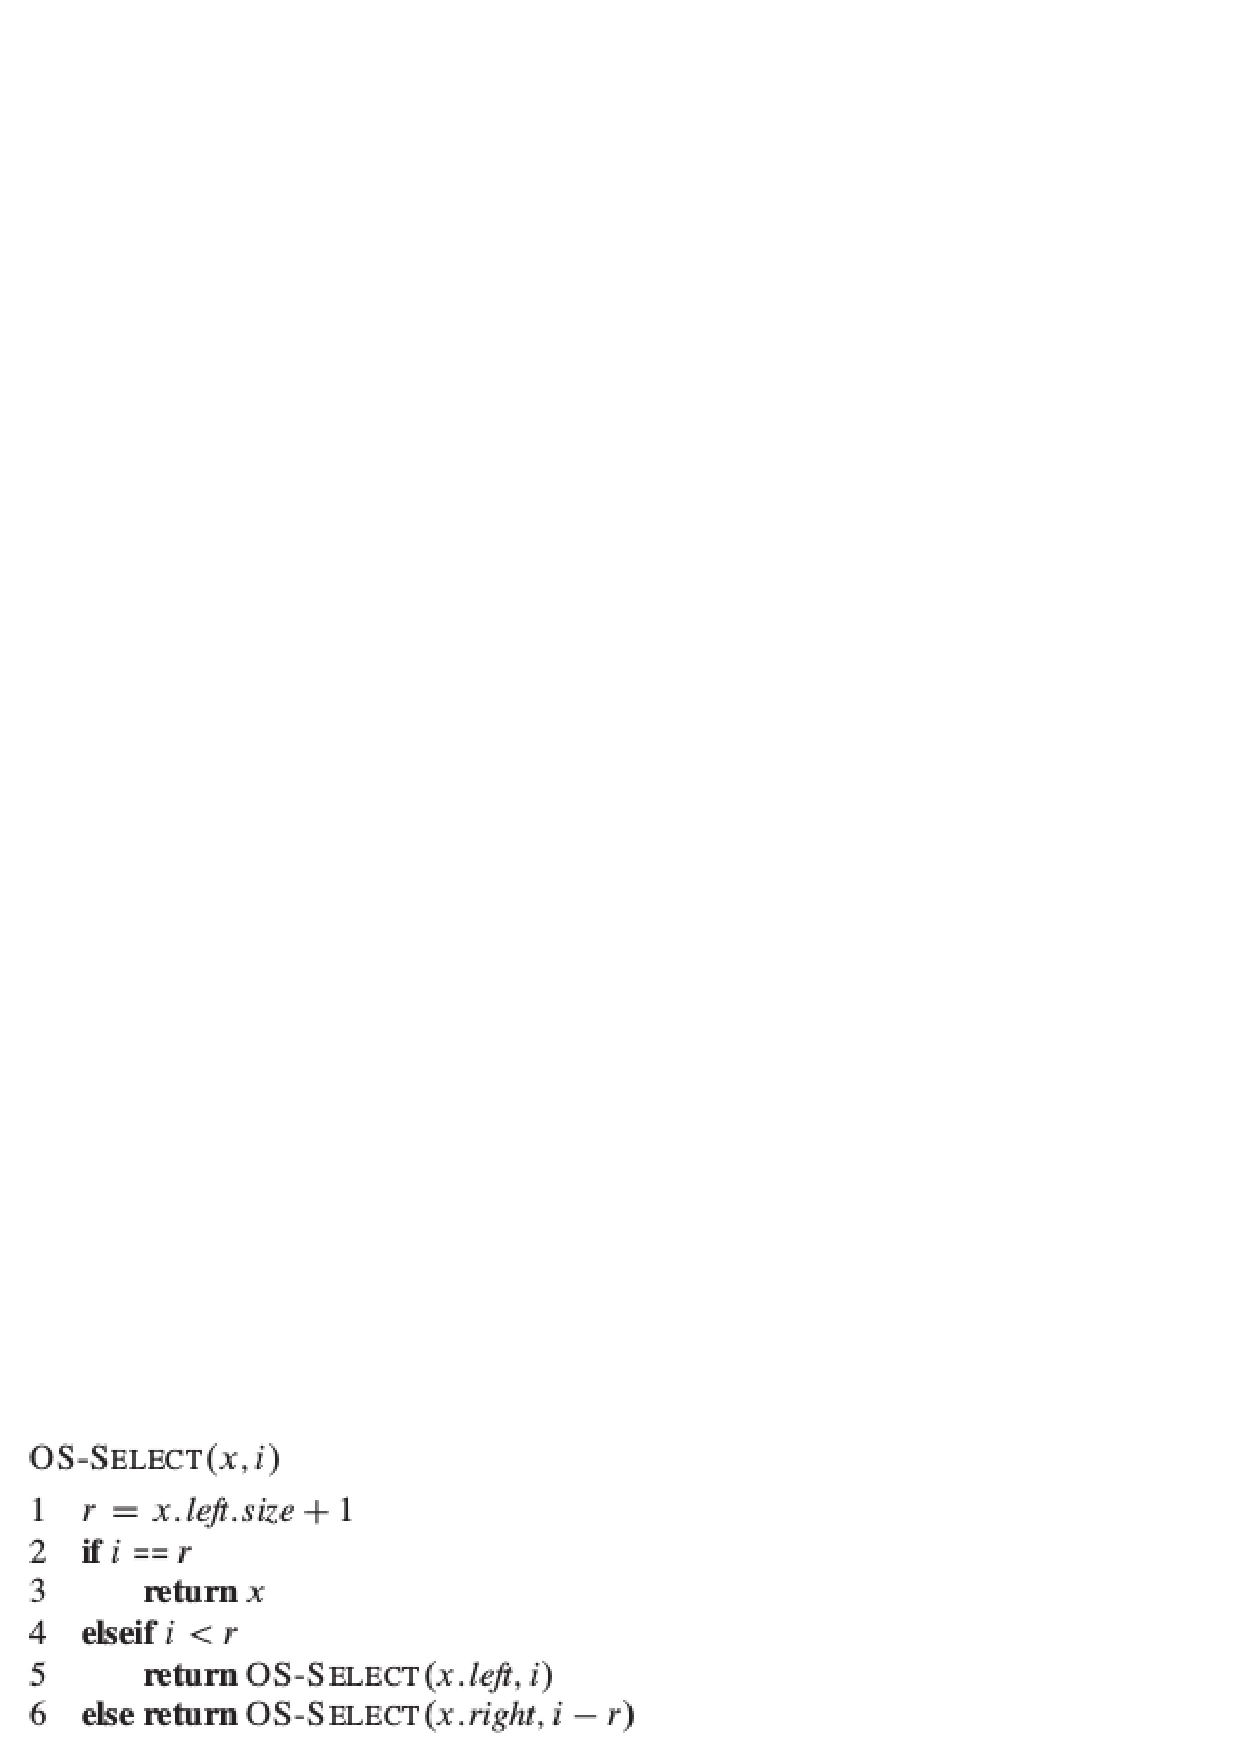
\includegraphics[scale = 0.5]{2.png}
  \caption{Resultado del programa}
 \end{figure}

 \item \textbf{La instrucción \textit{glLineWidth(3)}, permite cambiar el grosor de una línea. Añada otra línea de grosor diferente, al
 mismo tiempo, cambie el color de fondo y el color de la primera línea.}
 
 \begin{lstlisting}
#include <GL/glut.h>


void init(void){
    glClearColor(1.0,1.0,1.0,0.0);
    glMatrixMode(GL_PROJECTION);
    gluOrtho2D(0.0,250.0,0.0,150.0);
}

void line1(void){
    glBegin(GL_LINES);
        glVertex2i(10,145);
        glVertex2i(180,15);
    glEnd();
}

void line2(void){
    glBegin(GL_LINES);
        glVertex2i(60,145);
        glVertex2i(230,15);
    glEnd();
}

void lineSegment(void){
    glClear(GL_COLOR_BUFFER_BIT);

    glColor3f(0.0,0.4,0.2);
    line1();
    glFlush();


    glLineWidth(3);
    glColor3f(1.0,0.0,0.0);
    line2();
    glFlush();

    glLineWidth(1);
    glColor3f(0.0,0.4,0.2);
    line1();
    glClearColor(0.8,0.8,0.8,0.0);
    glFlush();

    //glColor3f(1.0,0.0,0.0);
    
}

int main(int argc, char **argv)
{
    glutInit(&argc,argv);
    glutInitDisplayMode(GLUT_SINGLE | GLUT_RGB);
    glutInitWindowPosition(50,100);
    glutInitWindowSize(400,300);
    glutCreateWindow("Ejemplo");
    init();
    glutDisplayFunc(lineSegment);
    glutMainLoop();
}
 \end{lstlisting}
 
 \begin{figure}[H]
  \centering
  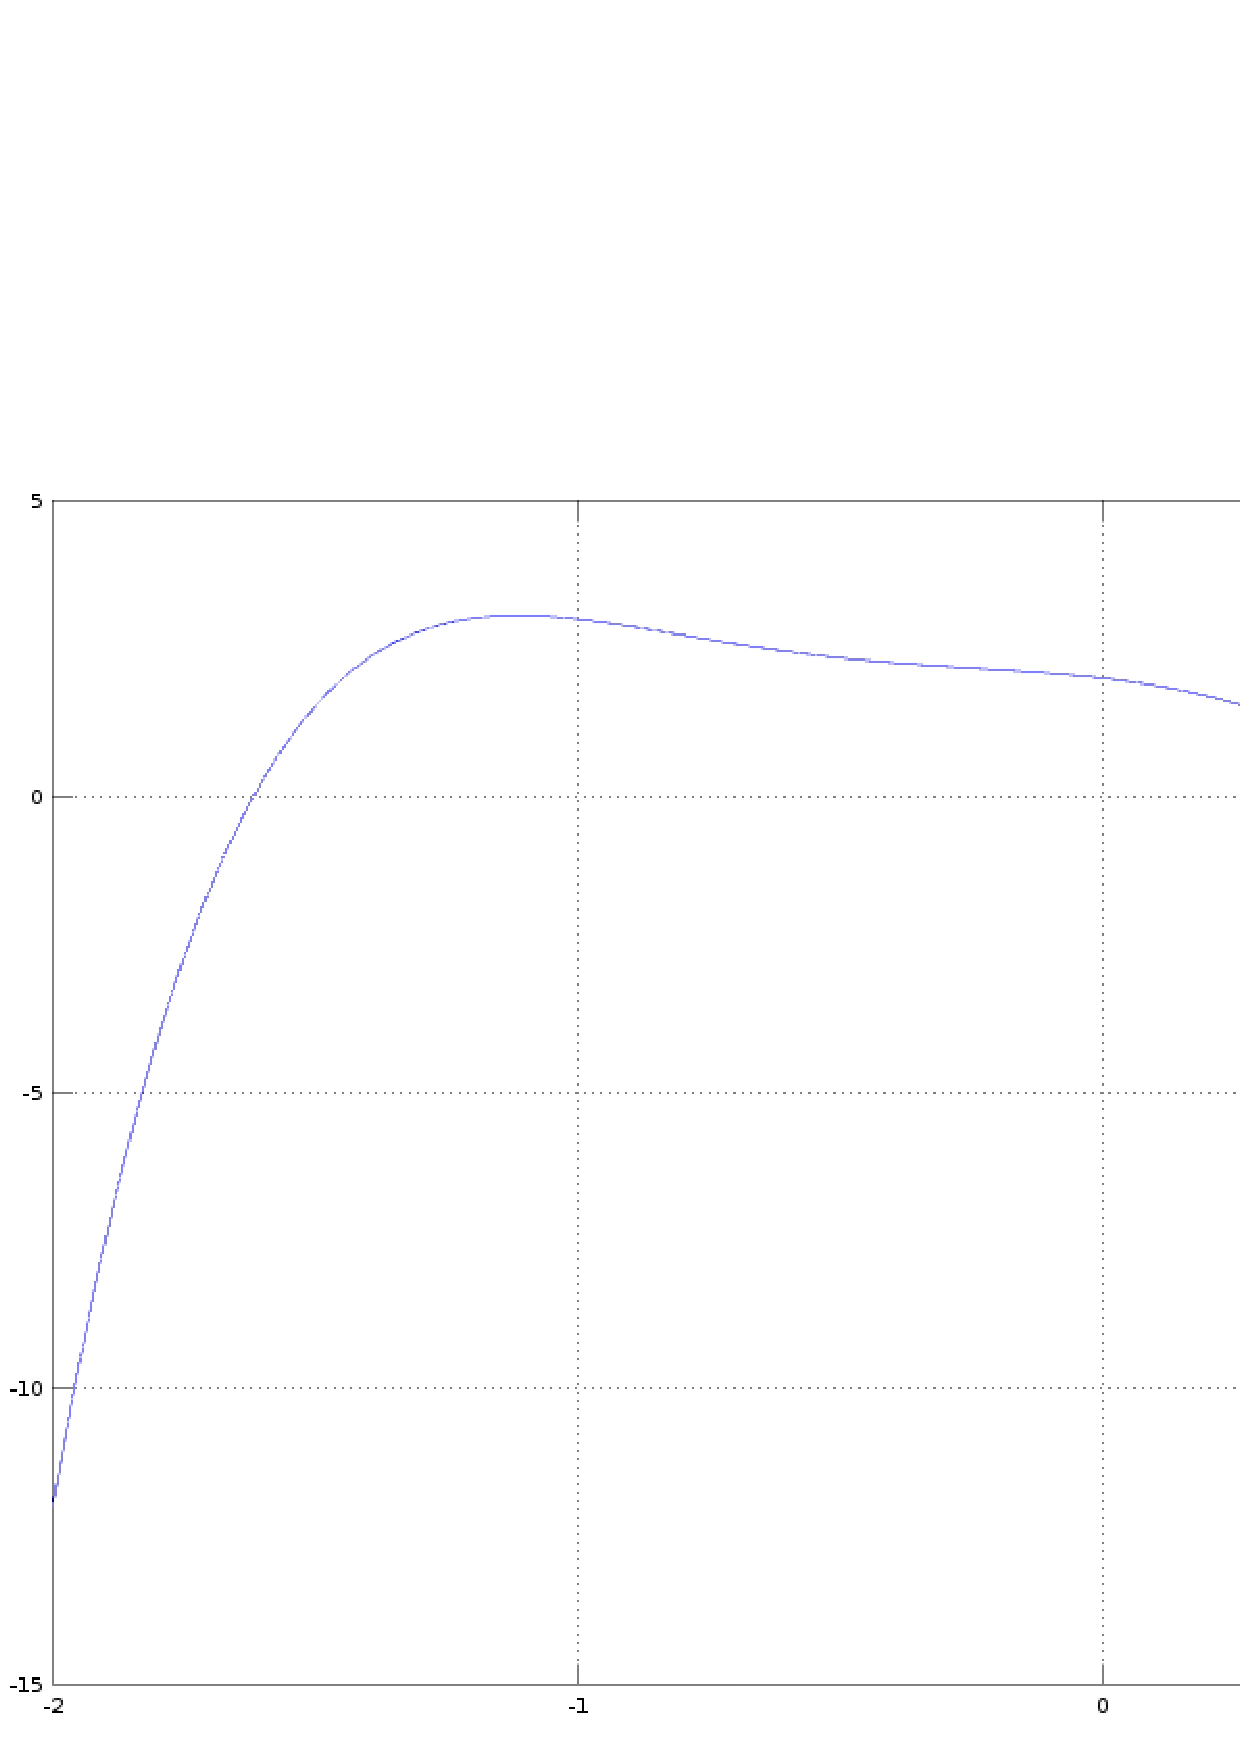
\includegraphics[scale = 0.5]{3.png}
  \caption{Resultado del programa}
 \end{figure}

 \item \textbf{Dibuje una casa utilizando líneas, considere que algunas pueden tener un color y grosor diferente}
 
 Se dibujan cuatro partes de la casa: la parte de abajo de la casa, el techo de la casa, la puerta de la casa, y las dos ventanas de la casa. A cada una 
 de estas partes se le puede cambiar el color y el grosor de las líneas. El tamaño de la casa depende de las variables \textit{anchoCasa} y \textit{altoCasa}.
 La posición de la casa depende de la variable \textit{puntoCentralPisoCasa}.
 
 \begin{lstlisting}
#include <GL/glut.h>
#include <iostream>
#include <tuple>

using namespace std;

typedef tuple<float,float> Point;

float anchoPantalla;
float altoPantalla;
Point puntoCentralPisoCasa;
float anchoCasa;
float altoCasa;

float grosorCasa = 3;
float grosorTecho = 3;
float grosorPuerta = 1;
float grosorVentanas = 1;


void init(void){
    glClearColor(1.0,1.0,1.0,0.0);
    glMatrixMode(GL_PROJECTION);
    gluOrtho2D(0.0,anchoPantalla,0.0,altoPantalla);
}

void drawLine(Point a, Point b){
    float x1;
    float x2;
    float y1;
    float y2;
    tie(x1,y1) = a;
    tie(x2,y2) = b;
    glBegin(GL_LINES);
        glVertex2i(x1,y1);
        glVertex2i(x2,y2);
    glEnd();
}


void display(void){
    glClear(GL_COLOR_BUFFER_BIT);
    float mitadAltoCasa = altoCasa / 2;
    float mitadAnchoCasa = anchoCasa / 2;
    float mitadMitadAnchoCasa = mitadAnchoCasa / 2;
    float mitadMitadAltoCasa = mitadAltoCasa / 2;
    float mitadMitadMitadAnchoCasa = mitadMitadAnchoCasa / 2;
    float mitadMitadMitadAltoCasa = mitadMitadAltoCasa / 2;
    float mitadMitadMitadMitadAltoCasa = mitadMitadMitadAnchoCasa / 2;
    float puntoCentralPisoCasaX;
    float puntoCentralPisoCasaY;
    tie(puntoCentralPisoCasaX,puntoCentralPisoCasaY) = puntoCentralPisoCasa;

    Point puntaTecho = make_tuple(puntoCentralPisoCasaX, puntoCentralPisoCasaY + altoCasa);
    Point paredSupIzq = make_tuple(puntoCentralPisoCasaX - mitadAnchoCasa,
        puntoCentralPisoCasaY + mitadAltoCasa);
    Point paredSupDer = make_tuple(puntoCentralPisoCasaX + mitadAnchoCasa,
        puntoCentralPisoCasaY + mitadAltoCasa);
    Point paredInfIzq = make_tuple(puntoCentralPisoCasaX - mitadAnchoCasa, 
        puntoCentralPisoCasaY);
    Point paredInfDer = make_tuple(puntoCentralPisoCasaX + mitadAnchoCasa, 
        puntoCentralPisoCasaY);

    glLineWidth(grosorCasa);
    glColor3f(1.0,0.0,0.0);
    drawLine(paredSupIzq,paredSupDer);
    drawLine(paredSupDer,paredInfDer);
    drawLine(paredInfDer,paredInfIzq);
    drawLine(paredInfIzq,paredSupIzq);
    glFlush();

    glLineWidth(grosorTecho);
    glColor3f(0.0,0.4,0.2);
    drawLine(paredSupIzq,puntaTecho);
    drawLine(paredSupDer,puntaTecho);
    glFlush();

    Point puertaSupIzq = make_tuple(puntoCentralPisoCasaX - mitadMitadAnchoCasa,
        puntoCentralPisoCasaY + mitadMitadAltoCasa);
    Point puertaSupDer = make_tuple(puntoCentralPisoCasaX + mitadMitadAnchoCasa,
        puntoCentralPisoCasaY + mitadMitadAltoCasa);
    Point puertaInfIzq = make_tuple(puntoCentralPisoCasaX - mitadMitadAnchoCasa,
        puntoCentralPisoCasaY);
    Point puertaInfDer = make_tuple(puntoCentralPisoCasaX + mitadMitadAnchoCasa,
        puntoCentralPisoCasaY);

    glLineWidth(grosorPuerta);
    glColor3f(0.5,0.35,0.05);
    drawLine(puertaSupDer,puertaSupIzq);
    drawLine(puertaSupIzq,puertaInfIzq);
    drawLine(puertaInfDer,puertaSupDer);
    glFlush();

    Point ventanaIzqSupIzq = make_tuple(puntoCentralPisoCasaX - (mitadMitadAnchoCasa + mitadMitadMitadAnchoCasa),
        puntoCentralPisoCasaY + mitadAltoCasa - mitadMitadMitadMitadAltoCasa);
    Point ventanaIzqSupDer = make_tuple(puntoCentralPisoCasaX - mitadMitadMitadAnchoCasa,
        puntoCentralPisoCasaY + mitadAltoCasa - mitadMitadMitadMitadAltoCasa);
    Point ventanaIzqInfDer = make_tuple(puntoCentralPisoCasaX - mitadMitadMitadAnchoCasa,
        puntoCentralPisoCasaY + mitadMitadAltoCasa + mitadMitadMitadMitadAltoCasa);
    Point ventanaIzqInfIzq = make_tuple(puntoCentralPisoCasaX - (mitadMitadAnchoCasa + mitadMitadMitadAnchoCasa),
        puntoCentralPisoCasaY + mitadMitadAltoCasa + mitadMitadMitadMitadAltoCasa);

    glLineWidth(grosorVentanas);
    glColor3f(0.196078,0.6,0.8);
    drawLine(ventanaIzqSupDer,ventanaIzqSupIzq);
    drawLine(ventanaIzqSupIzq,ventanaIzqInfIzq);
    drawLine(ventanaIzqInfIzq,ventanaIzqInfDer);
    drawLine(ventanaIzqInfDer,ventanaIzqSupDer);

    Point ventanaDerSupIzq = make_tuple(puntoCentralPisoCasaX + mitadMitadMitadAnchoCasa,
        puntoCentralPisoCasaY + mitadAltoCasa - mitadMitadMitadMitadAltoCasa);
    Point ventanaDerSupDer = make_tuple(puntoCentralPisoCasaX + (mitadMitadAnchoCasa + mitadMitadMitadAnchoCasa),
        puntoCentralPisoCasaY + mitadAltoCasa - mitadMitadMitadMitadAltoCasa);
    Point ventanaDerInfDer = make_tuple(puntoCentralPisoCasaX + (mitadMitadAnchoCasa + mitadMitadMitadAnchoCasa),
        puntoCentralPisoCasaY + mitadMitadAltoCasa + mitadMitadMitadMitadAltoCasa);
    Point ventanaDerInfIzq = make_tuple(puntoCentralPisoCasaX + mitadMitadMitadAnchoCasa,
        puntoCentralPisoCasaY + mitadMitadAltoCasa + mitadMitadMitadMitadAltoCasa);

    drawLine(ventanaDerSupDer,ventanaDerSupIzq);
    drawLine(ventanaDerSupIzq,ventanaDerInfIzq);
    drawLine(ventanaDerInfIzq,ventanaDerInfDer);
    drawLine(ventanaDerInfDer,ventanaDerSupDer);
    
    glFlush();

    
    
}

int main(int argc, char **argv)
{
    anchoPantalla = 400;
    altoPantalla = 300;
    anchoCasa = 50;
    altoCasa = 100;
    puntoCentralPisoCasa = make_tuple(anchoPantalla / 2, 10);   
    glutInit(&argc,argv);
    glutInitDisplayMode(GLUT_SINGLE | GLUT_RGB);
    glutInitWindowPosition(50,100);
    glutInitWindowSize(anchoPantalla, altoPantalla);
    glutCreateWindow("Ejemplo");


    init();
    glutDisplayFunc(display);
    glutMainLoop();
}
 \end{lstlisting}

 \begin{figure}[H]
  \centering
  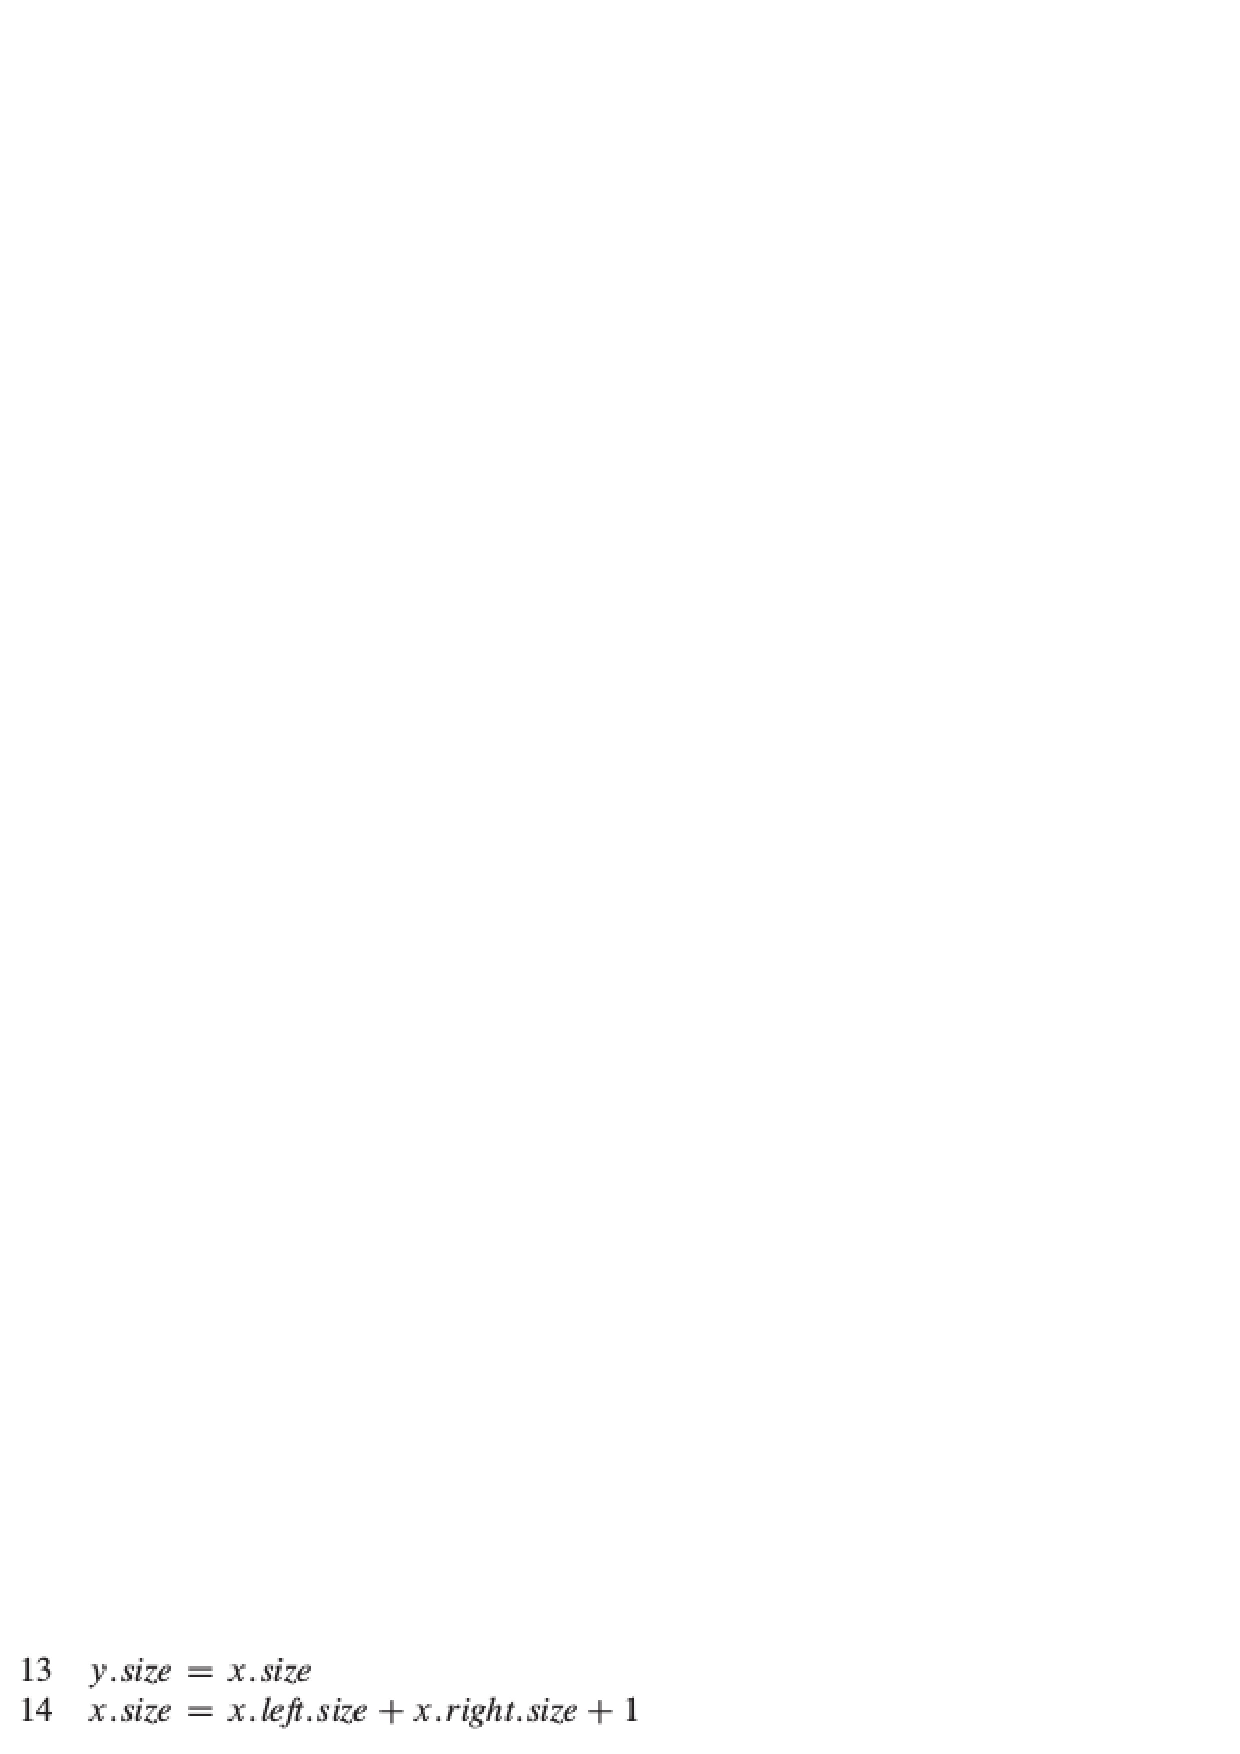
\includegraphics[scale = 0.5]{4.png}
  \caption{Resultado del Programa}
 \end{figure}
 
 \item \textbf{Plantee una estructura (clase, vector, matriz, etc) para salvar los datos de la pregunta 5}

Se utilizó una clase Casa para guardar todos los datos como el color y el grosor de cada parte. En el constructor se le pasa el tamaño y la posición de la casa.
También se inicializan los colores y el grosor por defecto. Si es que se quiere cambiar cualquiera de estos valores, se puede cambiar accesando a los miembros de la clase.
 
 
 \begin{lstlisting}
#include <GL/glut.h>
#include <iostream>
#include <tuple>

using namespace std;

typedef tuple<float,float> Point;

float anchoPantalla;
float altoPantalla;

typedef struct{
    float R;
    float G;
    float B;
}Color;

class Casa{
public:
    Casa(){};
    Casa(float ancho, float alto, float centralX, float centralY){
        puntoCentralPisoCasa = make_tuple(centralX,centralY);
        anchoCasa = ancho;
        altoCasa = alto;
        colorCasa.R = 1.0; colorCasa.G = 0.0; colorCasa.B = 0.0;
        colorTecho.R = 0.0; colorTecho.G = 0.4; colorTecho.B = 0.2;
        colorPuerta.R = 0.5; colorPuerta.G = 0.35; colorPuerta.B = 0.05;
        colorVentanas.R = 0.196078; colorVentanas.G = 0.6; colorVentanas.B = 0.8;
        grosorCasa = 1;
        grosorTecho = 1;
        grosorPuerta = 1;
        grosorVentanas = 1;
    }
    void drawCasa();
    Point puntoCentralPisoCasa;
    float anchoCasa;
    float altoCasa;
    Color colorCasa;
    Color colorTecho;
    Color colorPuerta;
    Color colorVentanas;
    float grosorCasa;
    float grosorTecho;
    float grosorPuerta;
    float grosorVentanas;
    
};


void init(void){
    glClearColor(1.0,1.0,1.0,0.0);
    glMatrixMode(GL_PROJECTION);
    gluOrtho2D(0.0,anchoPantalla,0.0,altoPantalla);
}

void drawLine(Point a, Point b){
    float x1;
    float x2;
    float y1;
    float y2;
    tie(x1,y1) = a;
    tie(x2,y2) = b;
    glBegin(GL_LINES);
        glVertex2i(x1,y1);
        glVertex2i(x2,y2);
    glEnd();
}

void Casa::drawCasa(){
    float mitadAltoCasa = altoCasa / 2;
    float mitadAnchoCasa = anchoCasa / 2;
    float mitadMitadAnchoCasa = mitadAnchoCasa / 2;
    float mitadMitadAltoCasa = mitadAltoCasa / 2;
    float mitadMitadMitadAnchoCasa = mitadMitadAnchoCasa / 2;
    float mitadMitadMitadAltoCasa = mitadMitadAltoCasa / 2;
    float mitadMitadMitadMitadAltoCasa = mitadMitadMitadAnchoCasa / 2;
    float puntoCentralPisoCasaX;
    float puntoCentralPisoCasaY;
    tie(puntoCentralPisoCasaX,puntoCentralPisoCasaY) = puntoCentralPisoCasa;

    Point puntaTecho = make_tuple(puntoCentralPisoCasaX, puntoCentralPisoCasaY + altoCasa);
    Point paredSupIzq = make_tuple(puntoCentralPisoCasaX - mitadAnchoCasa,
        puntoCentralPisoCasaY + mitadAltoCasa);
    Point paredSupDer = make_tuple(puntoCentralPisoCasaX + mitadAnchoCasa,
        puntoCentralPisoCasaY + mitadAltoCasa);
    Point paredInfIzq = make_tuple(puntoCentralPisoCasaX - mitadAnchoCasa, 
        puntoCentralPisoCasaY);
    Point paredInfDer = make_tuple(puntoCentralPisoCasaX + mitadAnchoCasa, 
        puntoCentralPisoCasaY);

    glLineWidth(grosorCasa);
    glColor3f(colorCasa.R,colorCasa.G,colorCasa.B);
    drawLine(paredSupIzq,paredSupDer);
    drawLine(paredSupDer,paredInfDer);
    drawLine(paredInfDer,paredInfIzq);
    drawLine(paredInfIzq,paredSupIzq);
    glFlush();

    glLineWidth(grosorTecho);
    glColor3f(colorTecho.R,colorTecho.G,colorTecho.B);
    drawLine(paredSupIzq,puntaTecho);
    drawLine(paredSupDer,puntaTecho);
    glFlush();

    Point puertaSupIzq = make_tuple(puntoCentralPisoCasaX - mitadMitadAnchoCasa,
        puntoCentralPisoCasaY + mitadMitadAltoCasa);
    Point puertaSupDer = make_tuple(puntoCentralPisoCasaX + mitadMitadAnchoCasa,
        puntoCentralPisoCasaY + mitadMitadAltoCasa);
    Point puertaInfIzq = make_tuple(puntoCentralPisoCasaX - mitadMitadAnchoCasa,
        puntoCentralPisoCasaY);
    Point puertaInfDer = make_tuple(puntoCentralPisoCasaX + mitadMitadAnchoCasa,
        puntoCentralPisoCasaY);

    glColor3f(colorPuerta.R,colorPuerta.G,colorPuerta.B);
    glLineWidth(grosorPuerta);
    drawLine(puertaSupDer,puertaSupIzq);
    drawLine(puertaSupIzq,puertaInfIzq);
    drawLine(puertaInfDer,puertaSupDer);
    glFlush();

    Point ventanaIzqSupIzq = make_tuple(puntoCentralPisoCasaX - (mitadMitadAnchoCasa + mitadMitadMitadAnchoCasa),
        puntoCentralPisoCasaY + mitadAltoCasa - mitadMitadMitadMitadAltoCasa);
    Point ventanaIzqSupDer = make_tuple(puntoCentralPisoCasaX - mitadMitadMitadAnchoCasa,
        puntoCentralPisoCasaY + mitadAltoCasa - mitadMitadMitadMitadAltoCasa);
    Point ventanaIzqInfDer = make_tuple(puntoCentralPisoCasaX - mitadMitadMitadAnchoCasa,
        puntoCentralPisoCasaY + mitadMitadAltoCasa + mitadMitadMitadMitadAltoCasa);
    Point ventanaIzqInfIzq = make_tuple(puntoCentralPisoCasaX - (mitadMitadAnchoCasa + mitadMitadMitadAnchoCasa),
        puntoCentralPisoCasaY + mitadMitadAltoCasa + mitadMitadMitadMitadAltoCasa);

    glColor3f(colorVentanas.R,colorVentanas.G,colorVentanas.B);
    glLineWidth(grosorVentanas);
    drawLine(ventanaIzqSupDer,ventanaIzqSupIzq);
    drawLine(ventanaIzqSupIzq,ventanaIzqInfIzq);
    drawLine(ventanaIzqInfIzq,ventanaIzqInfDer);
    drawLine(ventanaIzqInfDer,ventanaIzqSupDer);

    Point ventanaDerSupIzq = make_tuple(puntoCentralPisoCasaX + mitadMitadMitadAnchoCasa,
        puntoCentralPisoCasaY + mitadAltoCasa - mitadMitadMitadMitadAltoCasa);
    Point ventanaDerSupDer = make_tuple(puntoCentralPisoCasaX + (mitadMitadAnchoCasa + mitadMitadMitadAnchoCasa),
        puntoCentralPisoCasaY + mitadAltoCasa - mitadMitadMitadMitadAltoCasa);
    Point ventanaDerInfDer = make_tuple(puntoCentralPisoCasaX + (mitadMitadAnchoCasa + mitadMitadMitadAnchoCasa),
        puntoCentralPisoCasaY + mitadMitadAltoCasa + mitadMitadMitadMitadAltoCasa);
    Point ventanaDerInfIzq = make_tuple(puntoCentralPisoCasaX + mitadMitadMitadAnchoCasa,
        puntoCentralPisoCasaY + mitadMitadAltoCasa + mitadMitadMitadMitadAltoCasa);

    drawLine(ventanaDerSupDer,ventanaDerSupIzq);
    drawLine(ventanaDerSupIzq,ventanaDerInfIzq);
    drawLine(ventanaDerInfIzq,ventanaDerInfDer);
    drawLine(ventanaDerInfDer,ventanaDerSupDer);

    glFlush();
}




Casa casita;

void display(void){
    glClear(GL_COLOR_BUFFER_BIT);
    casita.drawCasa();
    glFlush();   
}


int main(int argc, char **argv)
{
    anchoPantalla = 400;
    altoPantalla = 300;
    int anchoCasa = 50;
    int altoCasa = 100;
    casita = Casa(anchoCasa, altoCasa, anchoPantalla / 2, 10);
    glutInit(&argc,argv);
    glutInitDisplayMode(GLUT_SINGLE | GLUT_RGB);
    glutInitWindowPosition(50,100);
    glutInitWindowSize(anchoPantalla, altoPantalla);
    glutCreateWindow("Ejemplo");


    init();
    glutDisplayFunc(display);
    glutMainLoop();
}
 \end{lstlisting}

 \item \textbf{¿Qué acciones sobre el código anterior (estructura de la pregunta 6) tendríamos que realizar para 
 trasladar la figura (casa} a otra posición?. Programe su idea.
 
 La idea que ya programé es basar la posición de toda la casa en función a la variable \textit{puntoCentralPisoCasa}. Este es el punto central del piso de la casa.
 Moviendo ese punto, se mueve toda la casa.
 
 \begin{figure}[H]
  \centering
  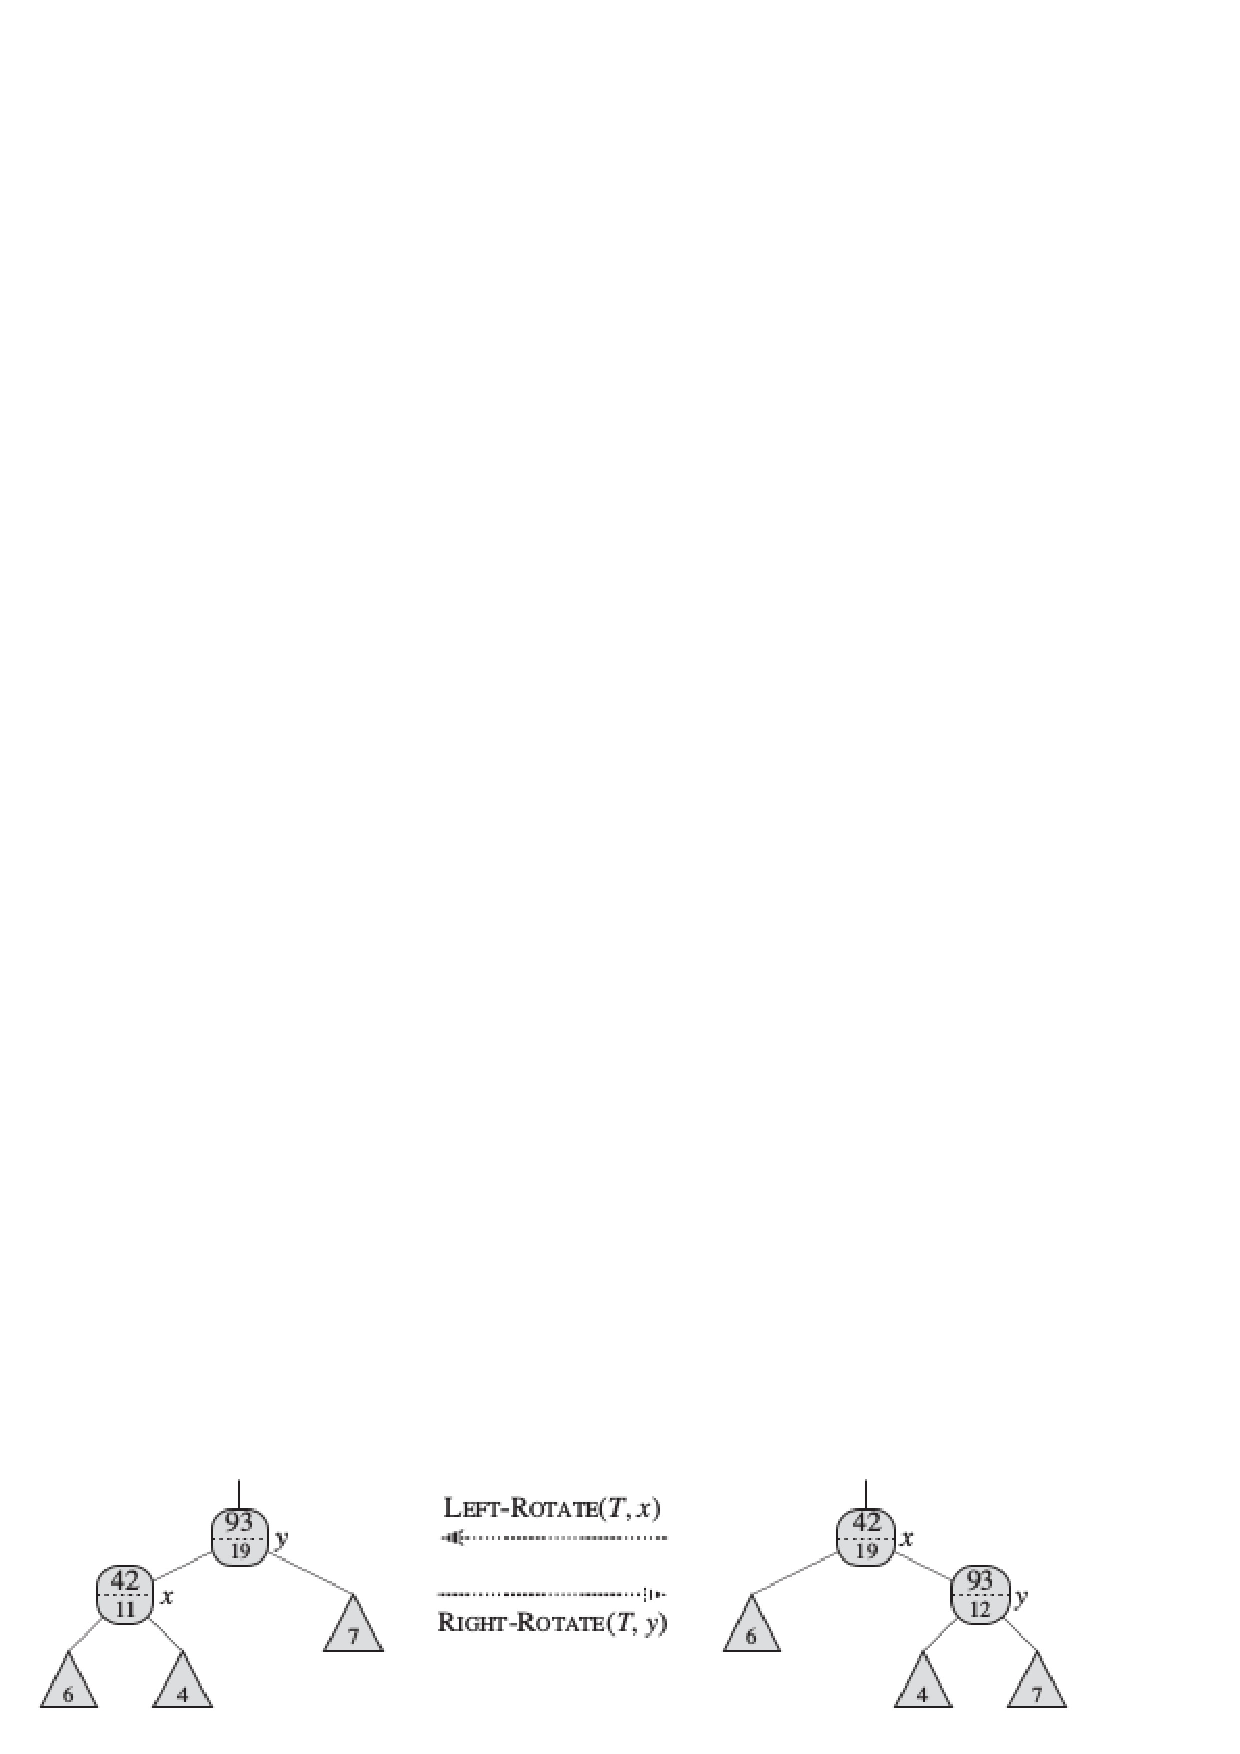
\includegraphics[scale = 0.5]{5.png}
 \end{figure}
 \begin{figure}[H]
  \centering
  \includegraphics[scale = 0.5]{6.png}
  \caption{Ejemplos de la casa movida}
 \end{figure}

 
 \item \textbf{¿Qué acciones sobre el código anterior (estructura de la pregunta 6) tendríamos que realizar para 
 escalar la figura (casa), es decir que sea más grande o más pequeña?. Programe su idea.}
 
 La idea que ya programé es basar el tamaño de toda la casa en función de las variables \textit{altoCasa} y \textit{anchoCasa}. El alto es desde el punto central del piso de
 la casa hasta la punta del techo, y el ancho es desde la esquina izquierda del piso de la casa hasta la esquina derecha del piso de la casa.
 
 \begin{figure}[H]
  \centering
  \includegraphics[scale = 0.5]{7.png}
  \caption{Ejemplo agrandando la casa}
 \end{figure}
 \begin{figure}[H]
  \centering
  \includegraphics[scale = 0.5]{8.png}
  \caption{Ejemplos achicando la casa}
 \end{figure}
 
 
 
\end{enumerate}


\end{document}

